\documentclass[svgnames]{beamer}
\mode<presentation>
\usefonttheme{serif}
\usecolortheme{dove}
\useinnertheme{rounded}
\setbeamercolor{item projected}{fg=black}
\setbeamertemplate{navigation symbols}{}

\usepackage[english]{babel}
\usepackage[latin1]{inputenc}
\usepackage{times}
\usepackage{amsmath}
\usepackage{amsfonts}
\usepackage{amssymb}
\usepackage{amsthm}
\usepackage{graphics}
\usepackage{multicol}
\usepackage{framed}
\usepackage{ulem}
\usepackage{ifthen}
\usepackage{tikz}
\usepackage{gastex}
\usepackage{ulem}
\usepackage{booktabs}

\newtheorem{hope}{Hope}
\newtheorem{observation}{Observation}
\newtheorem{conjecture}{Conjecture}

\def\checkmark{\tikz\fill[scale=0.4](0,.35) -- (.25,0) -- (1,.7) -- (.25,.15) -- cycle;} 

\newcommand{\MSO}{\mathrm{MSO}}
\newcommand{\N}{\mathbb{N}}
\newcommand{\B}{\mathbb{B}}
\newcommand{\F}{\mathbb{F}}
\newcommand{\ZFC}{\mathrm{ZFC}}
\newcommand{\Bool}{\mathcal{B}^+}
\newcommand{\Parity}{\textrm{Parity}}
\newcommand{\Buchi}{\textrm{B\"uchi}}
\newcommand{\Co}{\mathrm{Co}}
\newcommand{\A}{\mathcal{A}}

\newcommand{\rouge}[1]{\textcolor{Red}{#1}}

\renewcommand{\ULthickness}{1.2pt}

%%%%%%%%%%%%%%%%%%%%%%%%%%%%%%%%%%%%%%%%%%%%%%%%%%%%%%%%%%%%%%%%%%%%%%%%%%%%%%%
%%%%%%%%%%%%%%%%%%%% A non-original creation by Nathana�l Fijalkow and myself %

\setbeamertemplate{frametitle}{%
  \vskip-2pt%
  \begin{beamercolorbox}[rightskip=2cm,leftskip=1em,dp=1ex,wd=12.8cm]{frametitle}%
    \vskip2pt%
    \usebeamercolor{frametitle}%
    \begin{tikzpicture}[scale=1]%
      \useasboundingbox (0,0) rectangle (0,0); %(-1,-1) rectangle (1,1);%
      \ifthenelse{\insertframenumber<\inserttotalframenumber}%
      { % uncomplete tart

        \pgfmathsetmacro{\aimangle}{90-(\insertframenumber*360/\inserttotalframenumber)}
        \fill [fill=frametitle.fg,thin, color=gray!50,draw=black] (11.8,.2) -- (11.8,.6) arc (90:\aimangle:0.4) -- cycle;%

      }{ % the full tart
        \fill[fill=frametitle.fg,thin, color=gray!50,draw=black] (11.8,0.2) circle (.4);%
      }%
      \fill[fill=frametitle.fg,thin, color=white,draw=black] (11.8,0.2) circle (.3);%
      \node at (11.8, .2) [black,circle]{\normalsize\insertframenumber};

    \end{tikzpicture}
    \insertframetitle%
    \vskip2pt%
  \end{beamercolorbox}%
}
%%%%%%%%%%%%%%%%%%%%%%%%%%%%%%%%%%%%%%%%%%%%%%%%%%%%%%%%%%%%%%%%%%%%%%%%%%%%%%%


\setbeamertemplate{blocks}[rounded]%
\setbeamercolor{block title}{bg=normal text.bg!90!black}
\setbeamercolor{block body}{bg=normal text.bg!95!black}

\AtBeginSection[]
{
\addtocounter{framenumber}{-1}
  \begin{frame}<beamer>{Outline}
    \tableofcontents[currentsection]
  \end{frame}
}

\AtBeginSubsection[]
{
\addtocounter{framenumber}{-1}
  \begin{frame}<beamer>{Outline}
    \tableofcontents[currentsection,currentsubsection]
  \end{frame}
}

\begin{document}

\addtocounter{framenumber}{-1}

\title{Logical Formalisms Expressing\\Boundedness Properties\\over Infinite Trees}
\author{Nathana\"el Fijalkow}
\institute{Institute of Informatics, Warsaw University -- Poland 
\and LIAFA, Universit\'e Paris 7 Denis Diderot -- France}
\date{GT Jeux, January 24th, 2014}

\begin{frame}
\maketitle
\end{frame}

\section{Introduction}

\begin{frame}{Logics over infinite (binary) trees}
A tree:
\begin{figure}[!ht]
\begin{center}
\begin{picture}(50,40)(0,0)
	\gasset{Nh=5,Nw=5,Nframe=n,fillcolor=LightBlue}

	\node(v_0)(25,30){$a$}
	\node(v_1)(10,20){$b$}
	\node(v_2)(40,20){$a$}
	\node(v_3)(0,10){$b$}
	\node(v_4)(20,10){$a$}
	\node(v_5)(30,10){$b$}
	\node(v_6)(50,10){$b$}

	\drawedge(v_0,v_1){}
	\drawedge(v_0,v_2){}
	\drawedge(v_1,v_3){}
	\drawedge(v_1,v_4){}
	\drawedge(v_2,v_5){}
	\drawedge(v_2,v_6){}

	\put(-1,0){$\begin{huge}\vdots\end{huge}$}
	\put(19,0){$\begin{huge}\vdots\end{huge}$}
	\put(29,0){$\begin{huge}\vdots\end{huge}$}
	\put(49,0){$\begin{huge}\vdots\end{huge}$}
\end{picture}
\end{center}
\end{figure}

A logical property: 
\begin{center}
``for all nodes $a$, there are finitely many nodes \textit{below it}\\
that contain a branch with infinitely many $b$'s''
\end{center}
\end{frame}

\begin{frame}{Rabin's theorem}
\begin{small}
The variables $x,y,\ldots$ are interpreted by nodes, $X,Y,\ldots$ by sets of nodes.
\end{small}
\pause

Atomic formul\ae:
$$a(x) \quad \mid \quad x \in X \quad \mid \quad LeftChild(x,y) \quad \mid \quad RightChild(x,y)$$

Constructors:
$$\underbrace{\wedge,\vee,\neg}_{\text{boolean connectives}} \quad \mid \quad 
\underbrace{\exists x}_{\text{first-order}} \quad \mid \quad 
\underbrace{\exists X}_{\text{monadic second-order}}$$

\pause
\begin{theorem}[Rabin, 1969]
The following problem (called satisfiability problem) is decidable:
\begin{itemize}
	\item Instance: $\phi$ an MSO formula.
	\item Question: does there exist a tree $\bold t$ satisfying $\phi$?
\end{itemize}
\end{theorem}
\end{frame}

\begin{frame}{Extensions of Rabin's theorem}
\begin{center}
\begin{Huge}Can we go further?\end{Huge} 

\textit{i.e.} are there \textit{decidable} extensions of MSO
over infinite trees?
\vskip2em

Can we talk about the \textit{size} of sets?

About their \textit{asymptotic behaviour}?
\end{center}
\end{frame}

\begin{frame}{Some possible extensions}
\begin{itemize}
	\item ``$X$ is finite''\quad,\quad $|X| \ge 6$ \quad,\quad $|X| \equiv |Y| \bmod{9}$
	\begin{flushright}
		$\looparrowright$ already expressible in MSO
	\end{flushright}
\pause
	\item $|X| = |Y|$\quad,\quad$|X| \le |Y|$\quad,\quad$|X| = 2|Y|$
	\begin{flushright}
		$\looparrowright$ undecidable!
	\end{flushright}
\pause
	\item $\B X, \phi$, defined by
	$$\exists N \in \N,\ \forall X,\quad \phi(X) \Rightarrow |X| \le N$$
	\begin{flushright}
		$\looparrowright$ $\MSO + \B$ was proposed by Boja\'nczyk in 2004
	\end{flushright}

	\item $\ldots$ ?
\end{itemize}
\end{frame}

\begin{frame}{Bad news}
\begin{theorem}[Hummel, Skrzypczak and Toru\'nczyk, 2010]
$\MSO + \B$ is topologically \textit{very} hard
(reaches all levels of the projective hierarchy).
\end{theorem}
\pause
\begin{theorem}[Boja\'nczyk, Gogacz, Michalewski, Skrzypczak, 2014]
The decidability of $\MSO + \B$ over infinite trees cannot be proved in $\ZFC$.
\end{theorem}

(The decidability of $\MSO + \B$ over infinite words is still open.)
\pause

\begin{center}
\begin{Huge}
End of the story?
\pause

\rouge{Not quite!}
\end{Huge}
\end{center}
\end{frame}

\begin{frame}{Regular cost functions}
Colcombet investigated \textit{uniform} quantifications over bounds:
\vskip1em

Add ``$|X| \le N$'' to $\MSO$ formul\ae.

\begin{hope}[Colcombet, 2009]
The following problem (called boundedness problem) is decidable:
\begin{itemize}
	\item Instance: $\phi(N)$ a cost MSO formula.
	\item Question: $\exists N, \forall \bold t,\quad \bold t \models \phi[N]$?
\end{itemize}
\end{hope}

\pause
\vskip1em
\begin{theorem}[Colcombet 2009, Colcombet and Loeding 2011]
The boundedness problem is decidable for finite words, for infinite words and for finite trees.
\end{theorem}
\pause
\rouge{Wide open} for infinite trees!
It would solve a long-standing open problem (the decidability of the Mostowski index).
\end{frame}

\section{The three ingredients to prove Rabin's theorem}

\begin{frame}{A proof of Rabin's theorem, by Muller and Schupp}
Alternating parity automata:
$$\A = (Q,A,q_0,\delta,\Parity), \text{ where } \delta : Q \times A \rightarrow \underbrace{\Bool(Q \times Q)}_{\text{positive boolean combinations}}$$
\pause

\begin{figure}[ht]
\begin{minipage}{0.45\linewidth}
\centering

A tree $\bold t$ induces a two-player game between Eve and Adam:
\begin{itemize}
	\item Eve chooses disjunctions,
	\item Adam chooses conjunctions,
	\item Adam chooses directions.
\end{itemize}
$\bold t$ is accepted if Eve wins the acceptance game.
\end{minipage}
\hspace{0.5cm}
\begin{minipage}{0.45\linewidth}
\scalebox{1}{
	\begin{picture}(70,40)(0,0)
    \only<3,4>{\drawpolygon[linecolor=Red,linewidth=0.5,arcradius=3](0,18)(25,40)(50,18)}
	\only<4>{\drawpolygon[linecolor=Purple,linewidth=0.5,arcradius=3](25,3)(40,28)(55,3)}

	\gasset{Nframe=n}

	\node(q_0)(25,35){$q_0$}
	\only<3,4>{
	\node(q_1)(10,20){$p$}
	\node(q_2)(40,20){$r$}}
	
	\only<4>{
	\node(q_5)(30,5){$p$}
	\node(q_6)(50,5){$r$}}

	\gasset{Nh=5,Nw=5,Nframe=n,fillcolor=LightBlue}

	\node(v_0)(25,30){$a$}
	\node(v_1)(10,15){$b$}
	\node(v_2)(40,15){$a$}
	\node(v_3)(0,0){$b$}
	\node(v_4)(20,0){$a$}
	\node(v_5)(30,0){$b$}
	\node(v_6)(50,0){$b$}

	\drawedge(v_0,v_1){}
	\drawedge(v_0,v_2){}
	\drawedge(v_1,v_3){}
	\drawedge(v_1,v_4){}
	\drawedge(v_2,v_5){}
	\drawedge(v_2,v_6){}
	\end{picture}
}
\end{minipage}
\end{figure}
\end{frame}

\begin{frame}{A proof of Rabin's theorem, by Muller and Schupp}
We ``compile'' formul\ae\ into automata. 
Three difficulties:
\begin{itemize}
	\item complementation:
	\only<2,3,4>{$\looparrowright$ relies on the \rouge{determinacy of parity games}}

	\item existential quantification:
	\only<3,4>{$\looparrowright$ easy for non-deterministic automata}
	
	\item emptiness check:
	\only<3,4>{$\looparrowright$ easy for non-deterministic automata}
\end{itemize}

\pause\pause\pause
\vskip2em
Simulating alternating automata by non-deterministic ones relies on:
\begin{itemize}
	\item \rouge{determinization of parity automata over infinite words},
	\item \rouge{positional determinacy of parity games}.
\end{itemize}
\end{frame}

\begin{frame}{The three ingredients}

\begin{enumerate}
	\item Determinacy of parity games
	\item Determinization of parity automata over infinite words
	\item Positional determinacy of parity games
\end{enumerate}
\end{frame}

\begin{frame}{Towards cost MSO over infinite trees}
We need to generalize these three ingredients to \rouge{cost-parity games}:
\vskip1em
\begin{enumerate}
	\item Determinacy: \checkmark \quad (Borel determinacy takes over)
	\item Determinization: \checkmark \quad (history-deterministic automata fill in!)
	\item Positional determinacy: \quad only partial results...
\end{enumerate}
\end{frame}

\section{Towards finite-memory determinacy for cost-parity games}

\begin{frame}{Definition}
\begin{center}
\begin{multicols}{2}
\begin{picture}(40,60)(0,0)
	\gasset{Nw=8,Nh=8}
	
  	\rpnode[polyangle=45](1)(30,15)(4,5){}
  	\node(2)(20,30){}
  	\node(3)(40,30){}
  	\rpnode[Nmarks=i,iangle=180,polyangle=45](4)(0,30)(4,5){}
  	\rpnode[polyangle=45](5)(10,50)(4,5){}
  	\node(6)(10,10){}
  	\rpnode[polyangle=45](7)(30,50)(4,5){}

  	\drawedge(1,2){}
  	\drawedge[curvedepth=3](1,3){}
	\drawloop[loopangle=90](2){}
  	\drawedge(2,3){}
  	\drawedge(2,6){}
  	\drawedge[curvedepth=5](3,1){}
  	\drawedge(4,2){}
  	\drawedge[curvedepth=5](4,5){}
  	\drawedge[curvedepth=5](5,4){}
	\drawloop[loopangle=-90](6){}
  	\drawedge(7,5){}

\only<8,15>{
  	\rpnode[polyangle=45](1b)(30,15)(4,5){{\color{red}{$1$}}}
  	\node(2b)(20,30){{\color{blue}{$2$}}}
  	\node(3b)(40,30){{\color{red}{$3$}}}
  	\rpnode[Nmarks=i,iangle=180,polyangle=45](4b)(0,30)(4,5){{\color{red}{$3$}}}
  	\rpnode[polyangle=45](5b)(10,50)(4,5){{\color{blue}{$2$}}}
  	\node(6b)(10,10){{\color{blue}{$4$}}}
  	\rpnode[polyangle=45](7b)(30,50)(4,5){{\color{blue}{$0$}}}
}

\only<9,10,11,12,13,14,15>{
  	\drawedge(1,2){$i,\varepsilon$}
  	\drawedge[curvedepth=3](1,3){$\varepsilon,i$}
	\drawloop[loopangle=90](2){$i,i$}
  	\drawedge(2,3){$\varepsilon,\varepsilon$}
  	\drawedge[ELside=r](2,6){$i,r$}
  	\drawedge[curvedepth=5](3,1){$r,i$}
  	\drawedge(4,2){$\varepsilon,i$}
  	\drawedge[curvedepth=5](4,5){$\varepsilon,i$}
  	\drawedge[ELside=r,curvedepth=5](5,4){$i,i$}
	\drawloop[loopangle=-90](6){$\varepsilon,r$}
  	\drawedge[ELside=r](7,5){$i,\varepsilon$}
	}

\only<3,10>{\drawedge[AHLength=3,AHlength=4,linecolor=red,linewidth=0.7](4,2){}}
\only<5,12>{\drawedge[AHLength=3,AHlength=4,linecolor=red,linewidth=0.7](2,6){}}

\only<2,3,9,10>{\node[fillcolor=magenta,Nw=4,Nh=4](pebble)(0,30){}} 
\only<4,5,11,12>{\node[fillcolor=magenta,Nw=4,Nh=4](pebble)(20,30){}} 
\only<6,13>{\node[fillcolor=magenta,Nw=4,Nh=4](pebble)(10,10){}} 

\end{picture}
\begin{picture}(40,60)(0,0)
	\gasset{Nw=8,Nh=8}
	
\only<1,2,3,4,5,6>{
  	\node(Eve)(10,35){}
	\put(16,34){controlled by Eve}
  	\rpnode[polyangle=45](Adam)(10,25)(4,5){}
	\put(16,24){controlled by Adam}
	}

\only<8>{
	\begin{huge}
	\put(2,40){parity condition:}
	\put(-4,26){the minimal priority}
	\put(-4,18){seen infinitely often}
	\put(8,10){is even}
	\end{huge}
	}	

\only<9,10,11,12,13,14>{
	\begin{huge}
	\put(6,25){$\varepsilon: \textrm{nothing}$}
	\put(6,15){$i: \textrm{increment}$}
	\put(6,5){$r: \textrm{reset}$}
	\end{huge}
	}

\only<9,10>{
	\begin{huge}
	\put(10,50){$c_1 = 0$}
	\put(10,40){$c_2 = 0$}
	\end{huge}
}

\only<11,12>{
	\begin{huge}
	\put(10,50){$c_1 = 0$}
	\put(10,40){$c_2 = 1$}
	\end{huge}
}

\only<13,14>{
	\begin{huge}
	\put(10,50){$c_1 = 1$}
	\put(10,40){$c_2 = 0$}
	\end{huge}
}

\only<7,15>{
	\begin{huge}
	\put(12,36){parity}
	\put(15,28){and}
	\put(4,20){all counters}
	\put(3,12){are bounded}
	\end{huge}
}

\end{picture}
\end{multicols}
\end{center}
\end{frame}

\begin{frame}{Uniform versus non-uniform quantification}
Eve wins means:

\begin{figure}[ht]
\begin{minipage}[b]{0.45\linewidth}
\centering
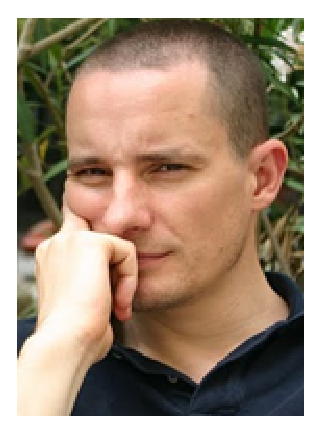
\includegraphics[width=19mm]{mikolaj}

$\exists \sigma$ (strategy for Eve),

$\forall \pi$ (paths), 

\rouge{$\exists N \in \N$},

\end{minipage}
\hspace{0.5cm}
\begin{minipage}[b]{0.45\linewidth}
\centering
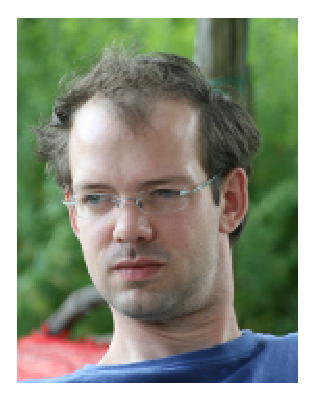
\includegraphics[width=20mm]{thomas}

\rouge{$\exists N \in \N$},

$\exists \sigma$ (strategy for Eve),

$\forall \pi$ (paths),
\end{minipage}
\end{figure}
\begin{center}
$\pi$ satisfies parity
and each counter is bounded by $N$.
\end{center}

\pause
\begin{figure}[ht]
\begin{minipage}[b]{0.45\linewidth}
\centering

non-uniform

$(\MSO + \B)$
\end{minipage}
\hspace{0.5cm}
\begin{minipage}[b]{0.45\linewidth}
\centering

uniform

$(\mathrm{cost}\ \MSO)$
\end{minipage}
\end{figure}
\end{frame}

\begin{frame}{Colcombet's Conjecture}
Fix a game $G$ and assume Eve wins $B(N) \cap \Parity$.
\begin{observation}
Eve has a strategy \rouge{with $N$ memory states} to ensure $B(N) \cap \Parity$.
\end{observation}
\pause
\vskip1em
The conjecture involves a \rouge{trade-off} between memory and quality:
\begin{conjecture}
There exists a function $\alpha : \N \to \N$ and a constant $m \in \N$ such that
for all games:\\
\centering
if Eve wins $B(N) \cap \Parity$,\\
then she has a strategy \rouge{with $m$ memory states} to ensure $B(\rouge{\alpha(N)}) \cap \Parity$.
\end{conjecture}
\end{frame}

\begin{frame}{An easy instance of Colcombet's Conjecture}
\begin{theorem}
for all \rouge{finite} games $G$:\\
\centering
if Eve wins $B(N) \cap \Parity$,\\
then she has a strategy \rouge{with $2$ memory states} to ensure $B(\rouge{|G| \cdot N}) \cap \Parity$.
\end{theorem}
\end{frame}

\begin{frame}{Some results obtained so far}
\only<1>{
\begin{theorem}[Vanden Boom]
For infinite chronological games:
\begin{itemize}
	\item If Eve wins $B(N) \cap \Buchi$,
then she has a strategy with $2$ memory states to ensure $B(N) \cap \Buchi$.
	\item If Eve wins $\overline{B}(N) \cup \Buchi$,
then she has a strategy with $2$ memory states to ensure $\overline{B}(N) \cup \Buchi$.
\end{itemize}
\end{theorem}

\begin{corollary}[Vanden Boom]
Cost weak MSO is decidable.
\end{corollary}
}

\only<2>{
\begin{theorem}[``Folklore in the regular cost function community'']
For infinite chronological games without $\varepsilon$:
\begin{itemize}
	\item If Eve wins $B(N) \cap \Parity$,
then she has a strategy with $2$ memory states to ensure $B(N) \cap \Parity$.
	\item If Eve wins $\overline{B}(N) \cup \Parity$,
then she has a strategy with $2$ memory states to ensure $\overline{B}(N) \cup \Parity$.
\end{itemize}
\end{theorem}

\begin{corollary}
MSO + ``$|x-y| \le N$'' (called temporal cost MSO) is decidable.
\end{corollary}
}

\only<3>{
\begin{theorem}[F.,Horn,Kuperberg,Skrzypczak]
Colcombet's Conjecture holds for \rouge{thin tree} games (with non-elementary bounds).
\end{theorem}

\begin{corollary}
Cost MSO is decidable over thin trees.
\end{corollary}
}
\end{frame}

\begin{frame}{Conclusion}
To extend Rabin's theorem to cost MSO via Muller and Schupp's proof, 
the following three ingredients are required:
\vskip1em
\begin{enumerate}
	\item Determinacy of cost-parity games: \checkmark
	\item Determinization of cost-parity automata over infinite words: \checkmark
	\item Finite-memory determinacy for cost-parity games: \rouge{ongoing}
\end{enumerate}
\end{frame}
\end{document}

